\documentclass{article}

\title{Distributed low rank approximation}
\author{Kadin Zhang}
\date{15-851, Spring 2025}

\usepackage[dvipsnames]{xcolor}
\usepackage{tikz}
\usetikzlibrary{calc}
\usepackage{enumitem}
\usepackage{alltt}
\usepackage{amsfonts}
\usepackage{amsmath}
\usepackage{amssymb}
\usepackage{amsthm}
\usepackage{booktabs}
\usepackage{bm}
\usepackage{bbm}
\usepackage{caption}
\usepackage{graphicx}
\usepackage{mathrsfs}
\usepackage{mathdots}
\usepackage{mathtools}
\usepackage{microtype}
\usepackage{multirow}
\usepackage{soul}
\usepackage{empheq}
\usepackage{mdframed}

% mdframed environments remain unchanged:
\newmdenv[
  innerbottommargin = 4mm,
  middlelinewidth = 0.3mm,
  linecolor = darkgray,
  backgroundcolor=TealBlue!10,
  nobreak=true
]{boxexample}
\newenvironment{ex}{\boxexample\begin{eg}}{\end{eg}\endboxexample}

\newmdenv[
  innerbottommargin = 4mm,
  middlelinewidth = 0.3mm,
  linecolor = darkgray,
  backgroundcolor=Salmon!10,
  nobreak=true
]{boxtheo}

\newmdenv[
  innerbottommargin = 4mm,
  middlelinewidth = 0.3mm,
  linecolor = darkgray,
  backgroundcolor=Goldenrod!20,
  nobreak=true
]{boxdefinition}
\newenvironment{thm}{\boxtheo\begin{theo}}{\end{theo}\endboxtheo}
\newenvironment{boxdef}{\boxdefinition\begin{defi}}{\end{defi}\endboxtheo}

\newenvironment{enum}{\newblock\begin{enumerate}[label=(\alph*)]}{\end{enumerate}}
\newenvironment{statement}[1]{\smallskip\noindent\color{BrickRed} {\bf #1.}}{}
\newenvironment{prob}{\color{BrickRed}\begin{probinner}}{\end{probinner}}
\newenvironment{comments}{\color{BrickRed}\begin{commentinner}}{\end{commentinner}}
\usepackage{imakeidx}
\newcommand{\argmin}{\operatornamewithlimits{arg\,min}}
\newcommand{\argmax}{\operatornamewithlimits{arg\,max}}

\makeindex[intoc, title=Index]
\usepackage[pdftex,
  hidelinks,
  pdfauthor={Kadin Zhang},
  pdfsubject={},
  pdftitle={},
  pdfkeywords={}]{hyperref}
\renewcommand\printindex{}

% Set standard 1-inch margins using the geometry package.
\usepackage[margin=1in]{geometry}

% Theorem styles and macros:
\newtheoremstyle{definition}{}{}{}{}{\bfseries}{:}{.5em}{\thmname{#1}\thmnumber{ #2}\thmnote{ (\textcolor{darkgray}{#3})}}
\theoremstyle{definition}

\newtheorem*{aim}{Aim}
\newtheorem*{axiom}{Axiom}
\newtheorem*{claim}{Claim}
\newtheorem*{cor}{Corollary}
\newtheorem*{conjecture}{Conjecture}
\newtheorem*{commentinner}{Comments}
\newtheorem*{defi}{Definition}
\newtheorem*{eg}{Example}
\newtheorem*{exc}{Exercise}
\newtheorem*{fact}{Fact}
\newtheorem*{law}{Law}
\newtheorem*{lemma}{Lemma}
\newtheorem*{notation}{Notation}
\newtheorem*{prop}{Proposition}
\newtheorem*{question}{Question}
\newtheorem*{rrule}{Rule}
\newtheorem*{theo}{Theorem}
\newtheorem*{assumption}{Assumption}

\newtheorem*{remark}{Remark}
\newtheorem*{warning}{Warning}
\newtheorem*{exercise}{Exercise}

\newtheorem{nthm}{Theorem}[section]
\newtheorem{nlemma}[nthm]{Lemma}
\newtheorem{nprop}[nthm]{Proposition}
\newtheorem{ncor}[nthm]{Corollary}
\newtheorem{probinner}[nthm]{Problem}

\renewcommand{\labelitemi}{--}
\renewcommand{\labelitemii}{$\circ$}
\renewcommand{\labelenumi}{(\roman{*})}

\newcommand\qedsym{\hfill\ensuremath{\square}}
\def\st{\bgroup \ULdepth=-.55ex \ULset}

% Mathematics symbols and operator definitions:
\newcommand{\leb}{\text{Leb}}

\newcommand{\C}{\mathbb{C}}
\newcommand{\CP}{\mathbb{CP}}
\newcommand{\GG}{\mathbb{G}}
\newcommand{\N}{\mathbb{N}}
\newcommand{\F}{\mathbb{F}}
\newcommand{\Q}{\mathbb{Q}}
\newcommand{\R}{\mathbb{R}}
\newcommand{\RP}{\mathbb{RP}}
\newcommand{\T}{\mathbb{T}}
\newcommand{\Z}{\mathbb{Z}}
\renewcommand{\H}{\mathbb{H}}

\DeclarePairedDelimiter\parens{\lparen}{\rparen}
\DeclarePairedDelimiter\abs{\lvert}{\rvert}
\DeclarePairedDelimiter\norm{\lVert}{\rVert}
\DeclarePairedDelimiter\floor{\lfloor}{\rfloor}
\DeclarePairedDelimiter\ceil{\lceil}{\rceil}
\DeclarePairedDelimiter\braces{\lbrace}{\rbrace}
\DeclarePairedDelimiter\bracks{\lbrack}{\rbrack}
\DeclarePairedDelimiter\angles{\langle}{\rangle}

\DeclarePairedDelimiter\bigp{\Big(}{\Big)}
\DeclarePairedDelimiter\bigc{\Bigg\{}{\Bigg\}}
\DeclarePairedDelimiter\biga{\Bigg|}{\Bigg|}

\DeclareMathOperator{\poly}{poly}
\DeclareMathOperator{\polylog}{polylog}
\DeclareMathOperator{\size}{size}
\DeclareMathOperator{\sgn}{sgn}
\DeclareMathOperator{\dist}{dist}
\DeclareMathOperator{\vol}{vol}
\DeclareMathOperator{\spn}{span}
\DeclareMathOperator{\supp}{supp}
\DeclareMathOperator{\tr}{tr}
\DeclareMathOperator{\Tr}{Tr}
\DeclareMathOperator{\codim}{codim}
\DeclareMathOperator{\diag}{diag}

\DeclareMathOperator{\lcm}{lcm}
\DeclareMathOperator{\OPT}{OPT}
\DeclareMathOperator{\DFT}{DFT}
\DeclareMathOperator{\rank}{rank}
\DeclareMathOperator{\nul}{nul}
\DeclareMathOperator{\ord}{ord}
\DeclareMathOperator{\diam}{diam}
\DeclareMathOperator{\erf}{erf}
\DeclareMathOperator{\err}{err}
\newcommand{\eps}{\varepsilon}

\DeclareMathOperator{\adj}{adj}
\DeclareMathOperator{\Aut}{Aut}
\DeclareMathOperator{\Char}{char}
\DeclareMathOperator{\Hom}{Hom}
\DeclareMathOperator{\id}{id}
\DeclareMathOperator{\image}{image}
\DeclareMathOperator{\im}{im}
\newcommand{\Frob}{\mathrm{Frob}}

\newcommand{\bolds}[1]{{\bfseries #1}}
\newcommand{\cat}[1]{\mathsf{#1}}
\newcommand{\mc}[1]{\mathcal{#1}}
\newcommand{\ph}{\,\cdot\,}
\newcommand{\term}[1]{\emph{#1}\index{#1}}
\newcommand{\phantomeq}{\hphantom{{}={}}}

\DeclareMathOperator{\PoA}{PoA}
\DeclareMathOperator{\PoS}{PoS}
\DeclareMathOperator{\Ber}{Ber}
\DeclareMathOperator{\io}{i.o.}
\DeclareMathOperator{\ev}{ev}
\DeclareMathOperator{\U}{U}
\DeclareMathOperator{\betaD}{beta}
\DeclareMathOperator{\bias}{bias}
\DeclareMathOperator{\Bin}{Bin}
\DeclareMathOperator{\corr}{corr}
\DeclareMathOperator{\cov}{cov}
\DeclareMathOperator{\var}{var}
\DeclareMathOperator{\gammaD}{gamma}
\DeclareMathOperator{\mse}{mse}
\DeclareMathOperator{\multinomial}{multinomial}
\DeclareMathOperator{\Poisson}{Poisson}
\newcommand{\E}{\mathbf{E}}
\newcommand{\wto}{\rightharpoonup}
\newcommand{\dto}{\xrightarrow{\text{d}}}
\newcommand{\pto}{\xrightarrow{\text{p}}}
\newcommand{\ato}{\xrightarrow{\text{a.s.}}}

\let\P\relax
\newcommand{\P}{\mathbf{P}}
\let\Pr\relax
\DeclareMathOperator*{\Pr}{\mathbf{Pr}}

\let\Im\relax
\let\Re\relax

\makeatother


\begin{document}
\maketitle
{
\small
\setlength{\parindent}{0em}
\setlength{\parskip}{1em}
}
% \tableofcontents

\section{Distributed low rank approximation}

Suppose $A$ is a large matrix, for example a customer product matrix, that we want to store on $s$ servers. One way to split the matrix among the servers is to let 
\[
    A = A^1 +A^2 +\dots +A^s ,
\]
called an \emph{arbitrary partition model}. Alternatively, we have have a \emph{row partition model}, where 
\[
    A = \begin{bmatrix}
         A^1  \\
         A^2  \\
         \vdots \\
         A^s  \\
    \end{bmatrix}.
\]
Within the customer product model, this restricts customers to shopping at a single store. 

We will assume a coordinator communication model:
\begin{center}
    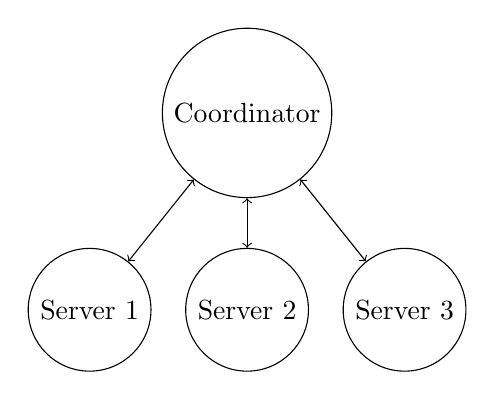
\begin{tikzpicture}[auto]
        % Coordinator node at the top center
        \node[circle, draw] (coord) at (0,0.5) {Coordinator};
    
        % Server nodes positioned manually below the Coordinator
        \node[circle, draw] (server1) at (-2,-2) {Server 1};
        \node[circle, draw] (server2) at (0,-2) {Server 2};
        \node[circle, draw] (server3) at (2,-2) {Server 3};
    
        % Bidirectional arrows connecting Coordinator to each Server
        \draw[<->] (coord) -- (server1);
        \draw[<->] (coord) -- (server2);
        \draw[<->] (coord) -- (server3);
    \end{tikzpicture}
\end{center}
Servers can communicate to any other server through the coordinator. This means we can simulate arbitrary point to point communication with at most twice the cost (along with the $\log s$ bits to specify a destination). 

\subsection{Projection intuition}
Suppose we have a $k$ dimensional subspace of $\R^d $ that we want to project onto. Let $W$ be a $d \times k$ matrix with orthogonal columns $w_i $ that span this subspace. These columns define the $k$ dimensional ``coordinate system'' of $W$. Then:
\begin{enum}
    \item $Wy$ takes a $\R^k $ vector $y$ in this coordinate system and transforms it back to $\R^d $. 
    \item $W^{\top} x$ takes a $\R^d $ vector $x$ and returns a vector of $\angles*{w_i ^{\top} x} $ (length of projection onto $i$th basis vector of $W$). This turns $x$ to the coordinates of $W$. 
    \item $WW^{\top}x$ takes a $\R^d $ vector, gets coordinates of projection onto $W$, then uses these coordinates to convert back to $\R^d $. 
\end{enum}

\subsection{Problem statement}

As input we have a $n\times d$ matrix $A$ split across our $s$ servers in either row partition or arbitrary partition format. Assume the entries of $A$ are $O(\log (nd))$-bit integers. 

For the arbitrary partition case, we have $A = A^1  +\dots +A^s $, and we want a rank $k$ approximation of $A$, $C$, such that 
\[
    \norm*{A - C}_{F} \leq (1+\eps )\norm*{A - A_k }_{F} ,
\]
where $A_k $ is the optimal rank $k$ approximation. In particular, we want to do this by determining a $k$ dimensional subspace $W$ that each server projects onto:
\[
    C = A^1 P_W  + A^2 P_W +\dots +A^s P_W . 
\]
Here, we represent $W$ as a $k\times d$ matrix where the rows are $\R^d $ basis vectors so that $P_W = W^{\top} W$ projects rows of $A^i $ onto $W$ (see above section). We would like to minimize total communication and computation, while keeping the amount of back-and-forth between each server and the coordinator (called round complexity) in $O(1)$. 

An example application is k-means clustering, where $A$ represents $n$ $d$-dimensional data points distributed across our servers in row partition format. With a good choice of subspace $W$ of $\R^d $, we could run clustering on the $n \times k$ matrix $AW^{\top} $ (working directly in the coordinates of our subspace), which is far more computationally efficient. 

\subsection{Work on distributed low rank approximation}
\cite{FSS} provided the first protocol for the row-partition model, requiring $O(sdk/\eps )$ real numbers of communication. It does not analyze the bit complexity of the communication, and can be slow since we are running SVD on both servers and the coordinator. 

\cite{KVW} improves this to achieve $O(sdk/\eps )$ communcation with good bit complexity on the arbitrary partition model, as well as better runtime. 

\cite{BWZ} achieves $O(skd) + \poly(sk/\eps )$ words of communication in the arbitrary partition model. This turns out to be optimal up to the lower order term $\poly(sk/\eps )$ (in general, we don't have too many servers, $k$ should be small since we're doing low rank approximation, and $\eps $ does not need to be too small). The lower bound is due to the fact that all $s$ servers need to learn the low rank space $W$. 

Some variants include: \cite{BLSWX} describes a protocol for distributed kernel low rank approximation, where we want an approximation to not the original data matrix $X$ but a kernel matrix where the rows are a kernel mapping of the original rows (often of higher dimension). \cite{WZ} describes a protocol for distributed low rank approximation of implicit matrices, where some function $f$ is applied elementwise to the matrix. \cite{BWZ} explores the case where $W$ is sparse and can be represented in better than $O(kd)$ parameters. 

\subsection{FSS protocol for row-partition model}

\begin{defi}[Coreset]
    Let $A$ be a $n\times d$ matrix with SVD $U\Sigma V^{\top} $. Define the \emph{coreset} of $A$ with a rank parameter $m$ as 
    \[
        \Sigma _m V_m ^{\top} ,
    \]
    where $\Sigma _m $ agrees with $\Sigma $ on the first $m$ diagonal entries and is $0$ elsewhere. In other words, we are taking the top $m$ principal directions scaled by their corresponding principal values, reducing the representation from $nd$ to $md$ parameters. 
\end{defi}

Think of the rows of $A$ as points in $\R^d $, and let $X$ be a $k$-dimensional subspace. 

\begin{center}
\begin{tikzpicture}[>=stealth]

    \draw[thick] (1,1) -- (6,6) node[pos=1, above right] {$X$};

    \coordinate (A1) at (2,5);
    \coordinate (A2) at (4,1);
    \coordinate (A3) at (6,4);

    \fill (A1) circle (2pt) node[above left] {$A_1$};
    \fill (A2) circle (2pt) node[below right] {$A_2$};
    \fill (A3) circle (2pt) node[above right] {$A_3$};

    \coordinate (P1) at (3.5,3.5);
    \fill (P1) circle (2pt) node[below right] {$A_1X$};

    \coordinate (P2) at (2.5,2.5);
    \fill (P2) circle (2pt) node[above left] {$A_2X$};

    \coordinate (P3) at (5,5);
    \fill (P3) circle (2pt) node[above left] {$A_3X$};

    \draw[dotted] (A1) -- (P1);
    \draw[dotted] (A2) -- (P2);
    \draw[dotted] (A3) -- (P3);

\end{tikzpicture}
\end{center}

The intuition for coresets is that the sum of squared distances from rows of $A$ to $X$ are roughly preserved when we substitute $A$ for $\Sigma _m V^{\top} $. To formalize this, note that the sum of squared distances from rows of $A$ to a subspace $X$ is the squared Frobenius norm of the projection onto $I - X$. We prove the below theorem. (sketching intuition?)

\begin{lemma}
    $\norm*{AB}_{F}^2   \leq \norm*{A}_{F}^2  \norm*{B}_2^2   $
\end{lemma}
\begin{proof}
    The $i$th row of $AB$ is the product between the $i$th row of $A$, $A_i $, and $B$. The squared length of this row is thus upper bounded by product of the squared length of $A_i $ with the largest singular value of $B$ squared, which is exactly the squared operator norm of $B$. So we can pull $\norm*{B}_{F} ^2 $ out of the Frobenius norm of the product. 

    Note that we can view $AB$ by columns $AB_{:, i} $ to achieve the result $\norm*{AB}_{F} ^2 \leq \norm*{A}_{2}^2  \norm*{B}_{F} ^2$. 
\end{proof}

\begin{thm}[]
    Let $Y = I-X$ be a projection matrix onto a $d-k$ dimensional subspace. Let $m = k + k/\eps $. Then 
    \[
        \norm*{AY}_{F}^2  \leq \norm*{\Sigma _m V^{\top} Y}_{F}^2  + c \leq (1+\eps )\norm*{AY}_{F} ^2,
    \]
    where $c = \norm*{A - A_m}_{F} ^2 $ (this doesn't depend on $Y$!). 
\end{thm}
\begin{proof}
    First, write $A = U\Sigma V^{\top} = U(\Sigma - \Sigma _m )V^{\top} + U\Sigma _m V^{\top} $, and use the Pythagorean theorem to obtain
    \[
        \norm*{AY}_{F} ^2 = \norm*{U\Sigma _m V^{\top} Y}_{F} ^2 + \norm*{U(\Sigma - \Sigma _m )V^{\top} Y}_{F} ^2 . 
    \]
    Since $U$ has orthonormal columns we may remove it from first norm. Since $Y$ is a projection matrix, its eigenvalues are at most $1$, so using the above lemma:
    \begin{align*}
        \norm*{U\Sigma _m V^{\top} Y}_{F} ^2 + \norm*{U(\Sigma - \Sigma _m )V^{\top} Y}_{F} ^2 &\leq \norm*{\Sigma _m V^{\top} Y}_{F} ^2 + \norm*{U(\Sigma - \Sigma _m )V^{\top}}_{F} ^2\\
        &= \norm*{\Sigma _m V^{\top} Y}_{F} ^2 + \norm*{A- A_m }_{F} ^2.
    \end{align*}
    This completes the first inequality. For the second inequality:
    \begin{align*}
        &\norm*{\Sigma _m V^{\top} Y}_{F} ^2 + \norm*{A- A_m }_{F} ^2 - \norm*{AY}_{F} ^2\\
        &= \norm*{\Sigma _m V^{\top} }_{F} ^2 - \norm*{\Sigma _m V^{\top} X}_{F}^2  + \norm*{A- A_m }_{F} ^2  - \norm*{A}_{F} ^2 + \norm*{AX}_{F} ^2\\
        &= \norm*{AX}_{F} ^2 - \norm*{\Sigma _m V^{\top} X}_{F}^2  \tag{Pythagorean on $(A-A_m ) + A_m = A$}\\
        &= \norm*{(\Sigma - \Sigma _m )V^{\top} X}_{F} ^2 \\
        &\leq \norm*{(\Sigma -\Sigma _m) V^{\top} }_2 ^2\norm*{X}_{F} ^2 \tag{lemma}\\
        &=  \sigma _{m+1} ^2 k \tag{$X$ is rank $k$ projection}\\
        &\leq \sigma _{m+1} ^2 (m - k)\eps \tag{$m = k + k/\eps $}\\
        &\leq  \eps \sum _{i = k+2} ^{m+1} \sigma _i ^2 \\
        &\leq \eps \norm*{A - A_k }_{F} ^2 \tag{$\norm*{A-A_k }_{F} ^2 = \sigma _{k+1}^2 +\dots +\sigma _{d}^2$}\\
        &\leq \eps \norm*{AY}_{F} ^2 \tag{optimality of $A_k $}. 
    \end{align*}
    Adding $\norm*{AY}_{F} ^2 $ to both sides completes the proof. 
\end{proof}

\begin{thm}[]
    The best rank $k$ approximation to a coreset is a good approximation of the best rank $k$ approximation to the original matrix. 
\end{thm}
\begin{proof}
    Suppose 
    \[
        Y' = \argmin_{Y} \norm*{\Sigma _m V^{\top} Y}_{F} ,
    \]
    i.e. $Y'$ is complement of the projection onto the best $k$-dimensional approximation to the coreset. Letting this approximation be $V_k $ (we can compute by SVD), take $Y' = I - V_k ^{\top}V_k $. Then, 
    \begin{align*}
        \norm*{AY'}_{F} ^2 &\leq \norm*{\Sigma _m V^{\top} Y'}_{F} ^2 +c\\
        &\leq \norm*{\Sigma _m V^{\top} Y^* }_{F} + c\\
        &\leq (1+\eps )\norm*{AY^* }_{F} ^2
        \\&=  (1+\eps )\norm*{A- A_k }_{F} ^2,
    \end{align*}
    where the first and third inequalities come from the proposition, and the second comes from optimality of $Y'$. So we can find a good rank $k$ subspace of $A$ operating only on the coreset $\Sigma _m V^{\top} $. 
\end{proof}

We need one last piece to state the FSS protocol. Suppose again we are in the row partition format with matrices $A^1 ,\dots , A^s $ and the servers compute coresets $\Sigma _m ^i V^{T, i} $ with constants $c_i $. Let $A$ be the matrix formed by concatenating the rows of the matrices. Summing over the theorem bound applied to each server, we have for any $d-k$ dimensional projection $Y$:
\[
    \sum_{i=1}^s (\norm*{\Sigma _m ^i V^{T, i} }_{F} ^2 + c_i) \leq (1+\eps ) \norm*{AY}_{F} ^2 . 
\]
Let $B$ be the matrix formed by concatenating the rows of the coresets, and suppose $\Sigma _m V^{\top} $ is a coreset for $B$. By coreset bound, for $c = \norm*{B - B_m }_{F}^2  $,
\[
    \norm*{\Sigma _m V^{\top} Y}_{F}^2  + c \leq \norm*{BY}_{F} ^2 . 
\]
Add $\sum_{i=1}^s c_i $ to both sides and use the last inequality to get
\[
    \norm*{\Sigma _m V^{\top} Y}_{F}^2  + c + \sum_{i=1}^s c_i \leq (1\pm O(\eps ))\norm*{AY}_{F} ^2 . 
\]
So the coreset of the concatenated coresets is a coreset of $A$ with constant $c+\sum_{i=1}^s c_i $. In conjunction with the last theorem, if we take the best rank $k$ approximation to this coreset by SVD, it will be close to the best rank $k$ approximation of $A$. This suffices to justify the FSS protocol:

\begin{defi}[FSS row-partition model protocol]
    Let $A$ be a $n\times d$ matrix distributed over $s$ servers each containing a $n_i \times d$ subset of its rows. Let $m = k/\eps +k$. 
    \begin{enum}
        \item Server $t$ sends $m$-coreset of $A^t $ and constant $c^t $ to the coordinator. 
        \item The coordinator concatenates the coresets and further computes a $m$-coreset of it along with constant $c$. It then returns this coreset $\Sigma _m V^{\top}  $ to each server. 
        \item The servers can now compute the best rank $k$ approximation of $\Sigma _m V^{\top} $ and project their points onto it. 
    \end{enum}
\end{defi}

% \subsubsection{KVW arbitrary partition model protocol}
% \begin{defi}[KVW protocol]
%     Let $S$ be a $k/\eps \times n$ random sketching matrix discussed earlier. We know that we can generate $S$ from a small seed. 
%     \begin{enum}
%         \item The coordinator sends a seed for $S$ to all servers. 
%         \item Server $t$ computes $SA^t $ and sends it to the coordinator. 
%         \item The coordinator sends $\sum_{t=1}^s SA^t = SA$ to the servers. 
%     \end{enum}
% \end{defi}

% Recall from the lecture on low rank approximation that there is a good rank $k$ approximation to $A$ within the rowspan of $SA$, so it's justified to project to $SA$ first and then find a low rank approximation. Naively, server $t$ could now project $A^t $ onto $SA$ and send it to the coordinator, but the communication cost would then depend on $n$. The next lecture will discuss how we address this.

\begin{thebibliography}{9}

\bibitem{FSS}
Dan Feldman, Melanie Schmidt, and Christian Sohler.
\newblock Turning big data into tiny data: constant-size coresets for k-means, PCA, and projective clustering.
\newblock \emph{SIAM Journal on Computing}, 2013.

\bibitem{KVW}
Ravi Kannan, Santosh Vempala, and David P. Woodruff.
\newblock Principal component analysis and higher principal components for distributed data.
\newblock In \emph{Proceedings of the 27th Conference on Learning Theory (COLT)}, pages 1040--1057, 2014.

\bibitem{BWZ}
Christos Boutsidis, David P. Woodruff, and Peilin Zhong.
\newblock Optimal principal component analysis in distributed and streaming models.
\newblock In \emph{Proceedings of the 48th Annual ACM Symposium on Theory of Computing (STOC)}, pages 236--249, 2016.

\bibitem{BLSWX}
Maria-Florina Balcan, Yingyu Liang, Le Song, David P. Woodruff, and Bo Xie.
\newblock \emph{Communication Efficient Distributed Kernel Principal Component Analysis}.
\newblock arXiv preprint arXiv:1503.06585, 2015.

\bibitem{WZ}
David P. Woodruff and Peilin Zhong.
\newblock Distributed Low Rank Approximation of Implicit Functions of a Matrix.
\newblock In \emph{Proceedings of the 32nd IEEE International Conference on Data Engineering (ICDE)}, 2016.

\end{thebibliography}


\end{document}